\documentclass[10pt,journal,compsoc]{IEEEtran}
\usepackage{amsmath,bm,mathtools}
\usepackage{tabularx,multirow,booktabs,blindtext}
\usepackage[T1]{fontenc}
\ifCLASSOPTIONcompsoc
\usepackage[nocompress]{cite}
\else
  % normal IEEE
  \usepackage{cite}
\fi

% correct bad hyphenation here
\hyphenation{op-tical net-works semi-conduc-tor}

\begin{document}

\title{A Two-step Kalman/Complementary Filter for Estimation of Vertical Position
Using an IMU-Barometer System}

\author{Jung Keun Lee
\IEEEcompsocitemizethanks{\IEEEcompsocthanksitem Department of Mechanical Engineering, Hankyong
National University
327 Jungang-ro, Anseong, Gyeonggi, 17579, Korea\protect\\
Corresponding author: jklee@hknu.ac.kr}
\thanks{(Received: April 15, 2016; Accepted : May 30, 2016)
This is an Open Access article distributed under the terms of the Creative
Commons Attribution Non-Commercial License(http://creativecommons.org/
licenses/bync/3.0) which permits unrestricted non-commercial use, distribution,
and reproduction in any medium, provided the original work is properly cited.}
\footnotesize \\Translated from Korean by Simon D. Levy (simon.d.levy@gmail.com)}\normalsize

% The paper headers
\markboth{Journal of Sensor Science and Technology 
Vol. 25, No. 3 (2016) pp. 202-207
http://dx.doi.org/10.5369/JSST.2016.25.3.202
SSN 1225-5475/eISSN 2093-7563}\%

\IEEEtitleabstractindextext{%
\begin{abstract}
Estimation of vertical position is critical in applications of sports science
and fall detection and also controls of unmanned aerial vehicles and
motor boats. Due to low accuracy of GPS(global positioning system) in the
vertical direction, the integration of IMU(inertial measurement unit) with
the GPS is not suitable for the vertical position estimation. This paper
investigates an IMU-barometer integration for estimation of vertical
position (as well as vertical velocity). In particular, a new two-step
Kalman/complementary filter is proposed for accurate and efficient
estimation using 6-axis IMU and barometer signals. The two-step filter is
composed of (i) a Kalman filter that estimates vertical acceleration via
tilt orientation of the sensor using the IMU signals and (ii) a
complementary filter that estimates vertical position using the barometer
signal and the vertical acceleration from the first step. The estimation
performance was evaluated against a reference optical motion capture
system. In the experimental results, the averaged estimation error of the
method was 19.7 cm while that of the raw barometer signal was 43.4
cm.  
\end{abstract}

\begin{IEEEkeywords}
Vertical position, Vertical acceleration, Kalman filter, Complementary filter, IMU(inertial measurement unit), Barometer
\end{IEEEkeywords}}


% make the title area
\maketitle


\IEEEdisplaynontitleabstractindextext
\IEEEpeerreviewmaketitle

\IEEEraisesectionheading{\section{Introduction}\label{sec:introduction}}

\IEEEPARstart{A}{ccurate} vertical position estimation for moving objects or humans is required
in various fields. For example, in the control of an unmanned aerial vehicle
(UAV) such as a drone, altitude is considered to be a kind of vertical
displacement [1], and vertical displacement such as a skier or snowboard is
required. In the case of severe spots, the vertical displacement estimation
using a portable sensor system can be used for analysis to improve light power
[2]. In order to overcome the space limitations of most motion capture systems
in tracking trajectories of moving objects GPS (global positioning system) IMU
(inertial measurement unit,  Inertial measurement device) has been attempted.
At this time, GPS provides displacement values that do not drift,
and inertial sensors provide high sampling rates, so that high sampling rate
and high accuracy displacement estimation are achieved through fusion of the
two sensors. However, the error of vertical direction displacement of GPS is
about 10 -- 20m, which is much lower than that of horizontal displacement [3]. 

As a countermeasure to this, a barometer can be utilized for vertical
displacement. However, the barometer is very noisy for use alone. Above all,
the barometer estimates the vertical displacement through the sensing of the
atmospheric pressure change. It responds sensitively to atmospheric conditions,
indoor / outdoor conditions, and even the degree of window opening, all of
which cause errors in the calculation of vertical displacement. Thus, similar
to IMU-GPS fusion, barometric-IMU convergence has been studied for
high-sampling rate and high-accuracy vertical displacement estimation [2,4-7].
In particular, IMU-barometer convergence is used in pedestrian navigation [8]
and fall detection [9] in terms of human monitoring.

Two approaches to the IMU and barometric convergence can be considered: tightly
coupled and loosely coupled [5]. The strong coupling method is effective in
modeling the noise of the two signals in a way that the signals of the IMU and
the barometer are fused from the beginning of the filter, but the system matrix
is ​​large and the calculation amount is large. On the other hand,
the weak coupling method uses a two-step filter and is used more frequently
because of convenience of application and efficiency of calculation. In this
case, the two-stage filter computes the vertical displacement using (i) the
first filter to calculate the attitude of the sensor using the IMU signal and
obtain the vertical acceleration through it, and (ii) the vertical acceleration
calculated from the barometer signal and the previous filter The second filter. 


Zihajehzadeh et al. [2] proposed a Kalman filter (KF) [10], which uses a 6-axis
IMU developed by this author (ie, a 3-axis accelerometer and a 3-axis
gyroscope) , And the Kalman filter, which sets the vertical displacement and
the vertical velocity as state variables, was used as the second filter.
Tanigawa et al. [7] applied the same Kalman filter as the first filter to the
Xsens three-dimensional posture calculation based on the 9-axis IMU (ie 6-axis
IMU + 3-axis geomagnetic sensor) All. Meanwhile, Sabatini and Genovese [5]
proposed an extended Kalman filter (Extended KF, EFK) that obtains quaternions
using 6-axis IMU As a first filter, use a complementary filter (CF) The second
filter was used. In addition, Son and Oh proposed [4] The EKF has claimed that
the IMU can be calibrated during the measurement by adding the accelerometer
bias and scale factor in addition to the vertical displacement and vertical
velocity as state variables, thereby improving the accuracy of posture and
vertical displacement estimation.

Among the above methods, all methods except [5] use a Kalman filter as the second filter,
for smoothing and smoothing effects.  However, the Kalman filter has a
disadvantage that the calculation amount is larger than that of the
complementary filter.

In this paper, the accurate vertical acceleration is estimated by using the
tilt estimation Kalman filter [10] adopted in [2] as the first filter, and a
new combination IMU - Barometer based

A two-stage Kalman / complementary filter is proposed. In addition, (1) the
effect of the accuracy of vertical acceleration estimation on the accuracy of
vertical displacement estimation in (1), and (2) the comparison between short
and long endpoints and estimation accuracy based on the complementary filter
and Kalman filter selection in the second stage. In this paper, we propose an
optimal vertical displacement estimation filter that combines the accuracy of
estimation and calculation efficiency.


\section{Estimation algorithm and verification experiment}

\subsection{Kalman filter for vertical acceleration estimation via posture estimation}

The Kalman filter for vertical acceleration estimation, which is the first
step, estimates the tilt as a vertical axis slope using an accelerometer and
gyroscope signal, which is a 6-axis IMU [10], and compensates for the
gravitational acceleration component in the accelerometer signal (See Fig. 1).

The signals of the gyroscope (G) and the accelerometer (A) were modeled as
follows:

\[\bm{s}_G = \prescript{S}{}{\bm{\omega}}+\bm{n}_G\tag{1.a}\]

\[\bm{s}_A = \prescript{S}{}{\bm{g}}+\prescript{S}{}{\bm{a}}+\bm{n}_G\tag{1.b}\]


\noindent where $\bm{\omega}$ is the angular velocity, $\bm{a}$ is the sensor
acceleration and $\bm{n}$ is the measurement noise. The superscript $S$ also
means that the vector is represented in the sensor coordinate system. In
equation (1.b), the sensor acceleration is modeled as a first-order Markov
chain process:

\[\prescript{S}{}{\bm{a}_t} = c_a\prescript{S}{}{\bm{a}_{t-1}}+\bm{\varepsilon}_{a,t}\tag{2}\]

\noindent where $c_a$ and $\bm{\varepsilon}_{a,t}$ are constant parameters and time-varying error terms of
the acceleration model, respectively.

The first filter estimates the tilt attitude expressed by
$\prescript{S}{}{\bm{Z}}$ as a state vector, and obtains the vertical
acceleration through the estimation. Where $\prescript{S}{}{\bm{Z}}$ is a
representation of the Z-axis unit vector of the inertial coordinate system I in
the sensor coordinate system and is part of a direction cosine matrix which is
a three-dimensional attitude matrix. First, the process model that updates the
state variable $x_1 (= \prescript{S}{}{\bm{Z}})$ over time is expressed as
follows from the strapdown integration associated with the angular velocity
measurement of the gyroscope:

\begin{figure}[!t]
\centering
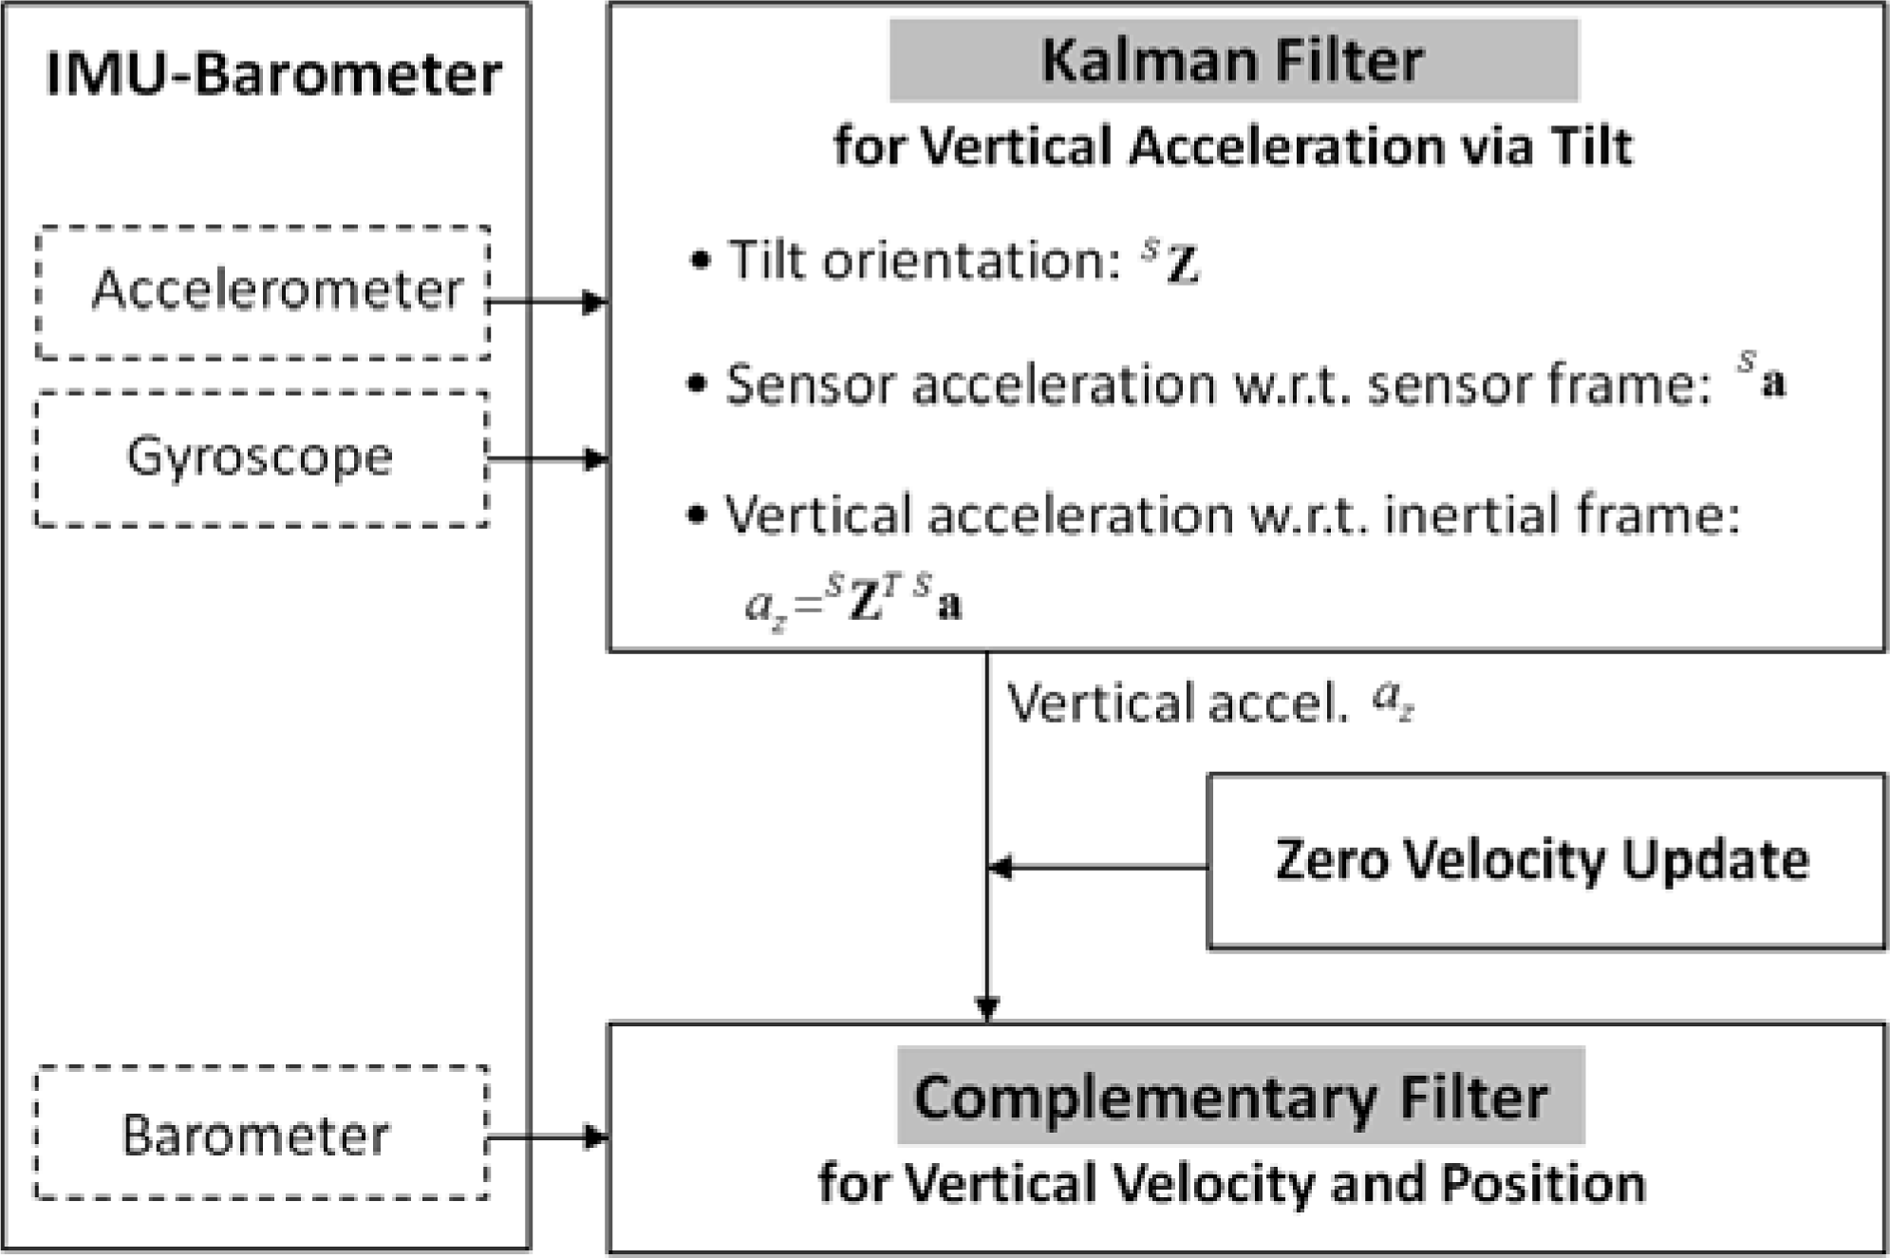
\includegraphics[width=2.5in]{fig1}
    \caption{Flowchart of the proposed two-step Kalman/complementary filter.}
\label{fig1}
\end{figure}


\[\bm{x}_{1,t}=\prescript{S}{}{\bm{Z}_t}=
(\bm{I}-\Delta t\bm{\tilde{s}}_{G,t-1})\prescript{S}{}{\bm{Z}_{t-1}}+\Delta t(-\prescript{\tilde{S}}{}{\bm{Z}_{t-1}})\bm{n}_G\tag{3}\]

Here, $\Delta t$ is the sampling interval and the tilde ($\tilde{~}$) denotes the outer matrix of
the vector, e.g., $\tilde{a} = [a \times]$.

The measurement model is a mixture of accelerometer signal and sensor acceleration model as follows:

\[\bm{s}_{A,t}-c_a\prescript{S}{}{\bm{a}^+_{t-1}}=g\prescript{S}{}{\bm{Z_t}}\prescript{S}{}{\bm{a}^-_{\varepsilon,t}}+\bm{n}_A\tag{4}\]


The following relation is applied in the above equation: 
$\prescript{S}{}{\bm{g}} = g\prescript{S}{}{\bm{Z}}$, 
$\prescript{S}{}{\bm{a}^-_{\varepsilon,t}} = \prescript{S}{}{\bm{a}^-_t} - \prescript{S}{}{\bm{a}_t}$, 
The superscripts $-$ and + mean the prior and the posterior, respectively.

From the equations (3) and (4) we obtain the following KF equation:

\[\bm{x}_{1,t} = \bm{\Phi}_{t-1}\bm{x}_{1,t-1} + \bm{w}_{t-1}\tag{5.a}\]

\[\bm{z}_t = \bm{H}_t \bm{x}_{1,t-1} + \bm{v}_t\tag{5.b}\]


\noindent where the transition matrix $\bm{\Phi}_{t-1}$ is $I - \Delta t
\bm{\tilde{s}}_{G,t-1}$; the process noise $\bm{w}_{t-1}$ is $\Delta t (-
\prescript{S}{}{\bm{\tilde{Z}}_{t-1}}) \bm{n}_G$; 
the measurement vector $\bm{z}_t$ is $\bm{s}_{A, t} - c_a \prescript{S}{}{\bm{a}}^+_{t-1}$;
The observation matrix $\bm{H}_t$ is $g\bm{I$}; and the measurement noise $\bm{v}_t$ is 
$-\prescript{S}{}{\bm{a}}_{\varepsilon,t} + \bm{n}_A$. The covariance matrix, 
$\bm{Q}_{t-1}$ (= $E [\bm{w}_{t-1} - \bm{w}^T{t-1}]$) and $\bm{M}_t$ (= $E [\bm{v}_t \bm{v}^T_t]$) 
for the progressive noise and the measured noise are as follows:

\[\bm{Q}_{t-1} = \Delta t^{2}\prescript{S}{}{\tilde{\bm{Z}}_{t-1}\Sigma_G}\prescript{S}{}{\tilde{\bm{Z}}_{t-1}}\tag{6.a}\]

\[\bm{M}_t = \Sigma_{acc} + \Sigma_A\tag{6.b}\]

\noindent where $E$ is the expectation operator, the covariance matrix $\Sigma_G$ for gyro
measurement noise is $\sigma^2_G I_3$; the covariance matrix $\Sigma_A$ for accelerometer
measurement noise is set to $\sigma_A \textbf{I}_3$; and $\sigma_G$ and $\sigma_A$ are noise standard
deviations. The covariance matrix $\Sigma_{acc}$ of the acceleration model error defined
by $E((\prescript{S}{}{\bm{a}}^+_{\varepsilon,t})(\prescript{S}{}{\bm{a}}^+_{\varepsilon,t})^T)$ 
is set to $3^{-1}c^2_a||\prescript{S}{}{\bm{a}}^+_{t-1}||\textbf{I}$.

Once $\prescript{S}{}{\bm{Z}}$ is obtained, the external acceleration
$\prescript{S}{}{\bm{a}}$ from the viewpoint of the sensor coordinate system is
obtained as  $\bm{s}_A-g\prescript{S}{}{\bm{Z}}$, and finally the $\bm{Z}$-direction
acceleration $\prescript{I}{}{a}_z$ from the viewpoint of the inertial coordinate system is
obtained by the following equation:

\[a_z(=\prescript{I}{}{a}_z)= \prescript{S}{}{\bm{a}}^T \prescript{S}{}{\bm{Z}}\tag{7}\]


\subsection{Complementary filter for vertical displacement estimation}

In the second step, a complementary filter, the vertical displacement 
$h_z (= \prescript{I}{}{h}_z)$ and the vertical velocity $v_z (= \prescript{I}{}{v}_z)$ 
are estimated using the vertical acceleration transmitted through the first Kalman filter and the barometric
signal.

The barometer pressure P can be converted to the vertical displacement h z by
the following equation [12].

\[h_z = 44330(1-(P/P_0)^{0.19})-h_{init}\tag{8}\]

\noindent where the unit of $h_z$ is m(eters) and $P_0$ is the atmospheric pressure at sea level
101,352 Pa(scals), and $h_{init}$ is the altitude of the starting point of
observation. In other words, $h_z$ in this paper is the variation of the vertical
displacement from the observation starting point.  Also, in this paper, based
on the highly transformed barometric pressure signal, the signal of the
barometer ($B$) is modeled as

\[s_B = h_z + n_B\tag{9}\]

The state vector $\bm{x}_2$ in the second filter, complementary filter, is [11]:

\[\bm{x}_2 = [h_z v_z]^T\tag{10}\]

Applying the introduced complementary filter is as follows:

\begin{equation}
\resizebox{.42 \textwidth}{!} 
{
$ 
\bm{x}_{2,t} = 
\begin{bmatrix} 1 & \Delta t \\ 0 & 1 \end{bmatrix} \bm{x}_{2,t-1} +
\begin{bmatrix} 1 & \Delta t / 2 \\ 0 & 1 \end{bmatrix} \bm{K}_c\Delta t \times \varepsilon_{h,t-1} +
\begin{bmatrix} \Delta t / 2 \\ 1 \end{bmatrix} \Delta v_{z,t-1}
$
}
\tag{11}
\end{equation}

Here, $\varepsilon_h$ is the difference between the barometric signal and the estimated value:

\[\varepsilon_{h,t-1} = s_{B,t-1} - h_{z,t-1}\tag{12}\]

And the velocity increment $\Delta v_z$ is $\Delta t \times a_Z$. In addition, the complementary filter gain (gain)
$\bm{K}_c$ is as follows:

\[\bm{K}_c = \begin{bmatrix}  \sqrt{2 (\sigma_{acc}/\sigma_B)} \\ \sigma_{acc}/\sigma_B \end{bmatrix} \tag{13}\]

\noindent where $\sigma_{acc}$ and $\sigma_B$ are the vertical acceleration estimate and the barometric signal,
respectively.   For references, this complementary filter has low-pass filter
characteristics of time constant $\tau = \sqrt{\sigma_B/\sigma_{acc}}$.


Prior to the above, the zero-velocity update (ZUPT) was applied.  Based
on the integration of noise, this is a technique to limit the drift error. When the
zero speed is detected (as follows), the speed is set to zero in preference to
the complementary filter integral (11):

\[v_{z,t} = \begin{cases} 0, if (|a_{z,\tau}|<0.1m/s^2 \forall_\tau\in[t-n\Delta t, t]) \\ Eq. (11)~otherwise \end{cases} \tag{14}\]

\noindent where $n$ is set to 12.

The overall configuration of the proposed two-stage Kalman / complementary filter is shown in Fig. 1.

\begin{figure}[!t]
\centering
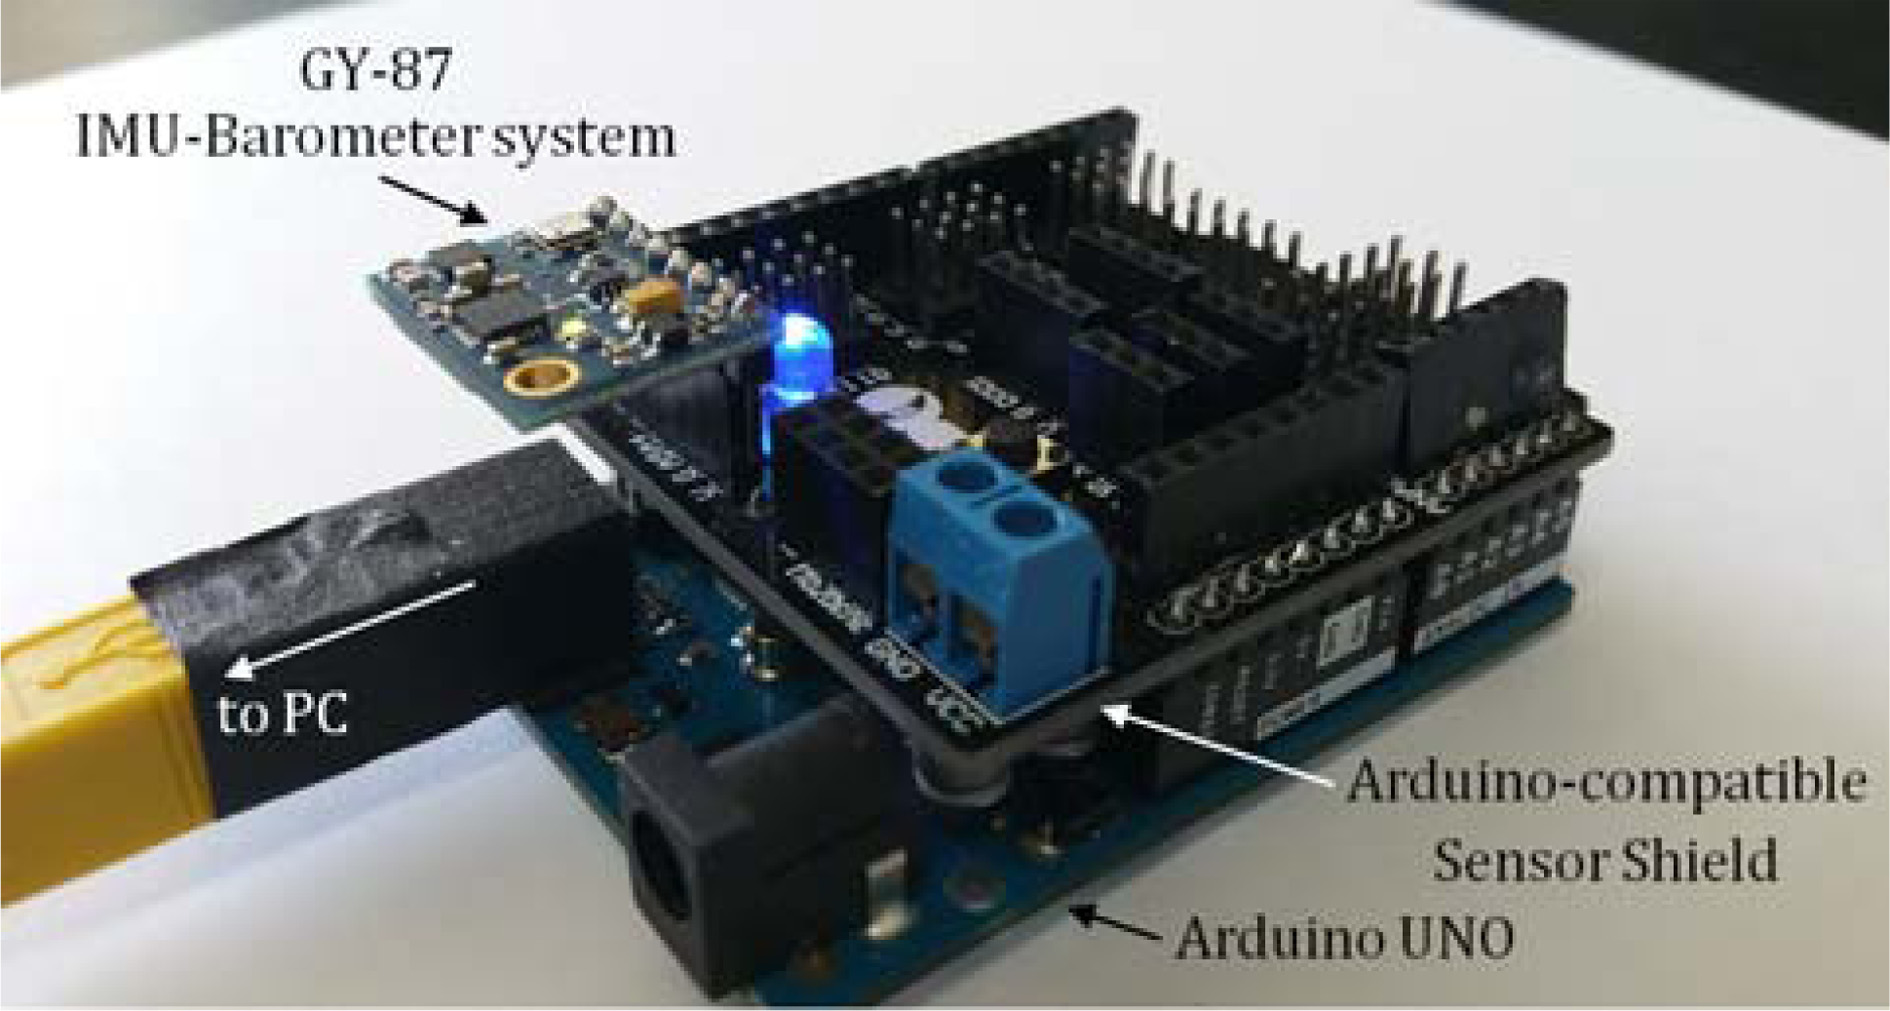
\includegraphics[width=2.5in]{fig2}
\caption{GY-87 IMU-Barometer and Arduino board system.}
\label{fig2}
\end{figure}


\subsection{Verification experiment}

A GY-87 modular system was used for verification experiments. The GY-87
consists of a 6-axis InvenSense MPU-6050 IMU (including accelerometer and
gyro), a 3-axis Honeywell HMC5883L geomagnetic sensor, and a Bosch BMP180
barometer, of which IMU and barometer were used for this experiment. Refer to
Table 1 for details.  The setup of the GY-87 is shown in Fig. 2 with Arduino
UNO R3 microcontroller (Arduino, Italy) and USB serial communication with the
PC and input to the filter.  The OptiTrack Flex13 optical motion capture system
(NaturalPoint, Inc. USA) of Figure 3 was used as a ground-truth reference to obtain
root mean square error (RMSE).  

In addition to the proposed two-stage Kalman / complementary filter method,
the following cases were compared and analyzed:

\begin{itemize}
\item The method of obtaining vertical acceleration: 
\begin{enumerate}
\item $a_{z,KF}$: the proposed method described in Section 2.1 using both accelerometer and gyroscope,
\item $a_{z,OPT}$: a method of obtaining vertical acceleration using a very accurate attitude obtained from the 
  Flex 13 camera system instead of the inertial sensor,
\item $a_{z,app}$: Approximate method using only accelerometer [13]. That is, $a_{z,app} = ||s_A|| - g$.
\end{enumerate}
\item How to find vertical displacement:
\begin{enumerate}
\item Using the complementary filter described in Section 2.2,
\item $[2]$ and [7] using Kalman filter.
\end{enumerate}
\end{itemize}

Five experiments were conducted as follows. Tests A to C are shown in Fig 3. As
shown in Fig. 3, these were performed in the indoor gymnasium, elevated above the
starting height by more than 3m. The optical marker was used only for the
reference value corresponding to the vertical displacement (That is, $a_{z,OPT}$
are not obtained through the reference value of the sensor attitude.) On the
other hand, Test D ~ E was lowered to within 1.5 m from the starting height.
To confirm the influence of $a_{z,KF}$ and $a_{z,OPT}$ on the vertical displacement
estimation, three additional markers were attached.  The test movements were as follows:
\begin{itemize}
    \item \textbf{Test A} Increased gradually from the starting height to around 3.5m.
         Waited for about 10 seconds before descending to the starting height again.
         XXX However, when the sensor is moved up or down and the sensor attitude changes by more than 
         45$^\circ$ XXX.  This experiment confirms the influence of vertical
         acceleration $a_{z,KF}$ and $a_{z,app}$ difference in attitude change in
         vertical displacement estimation.
    \item \textbf{Test B-C} Repeatedly ascending and descending by up to about 3m. Compared to Test B, 
        Test C had faster and more frequent ups and downs. This experiment
        confirms the influence of the movement speed on the vertical displacement
        estimation.
    \item \textbf{Test D} Cascaded steps up and down, then stop.
    \item \textbf{Test E} Observe the transition of the barometer signal at small altitude changes.
\end{itemize}

\begin{figure}[!t]
\centering
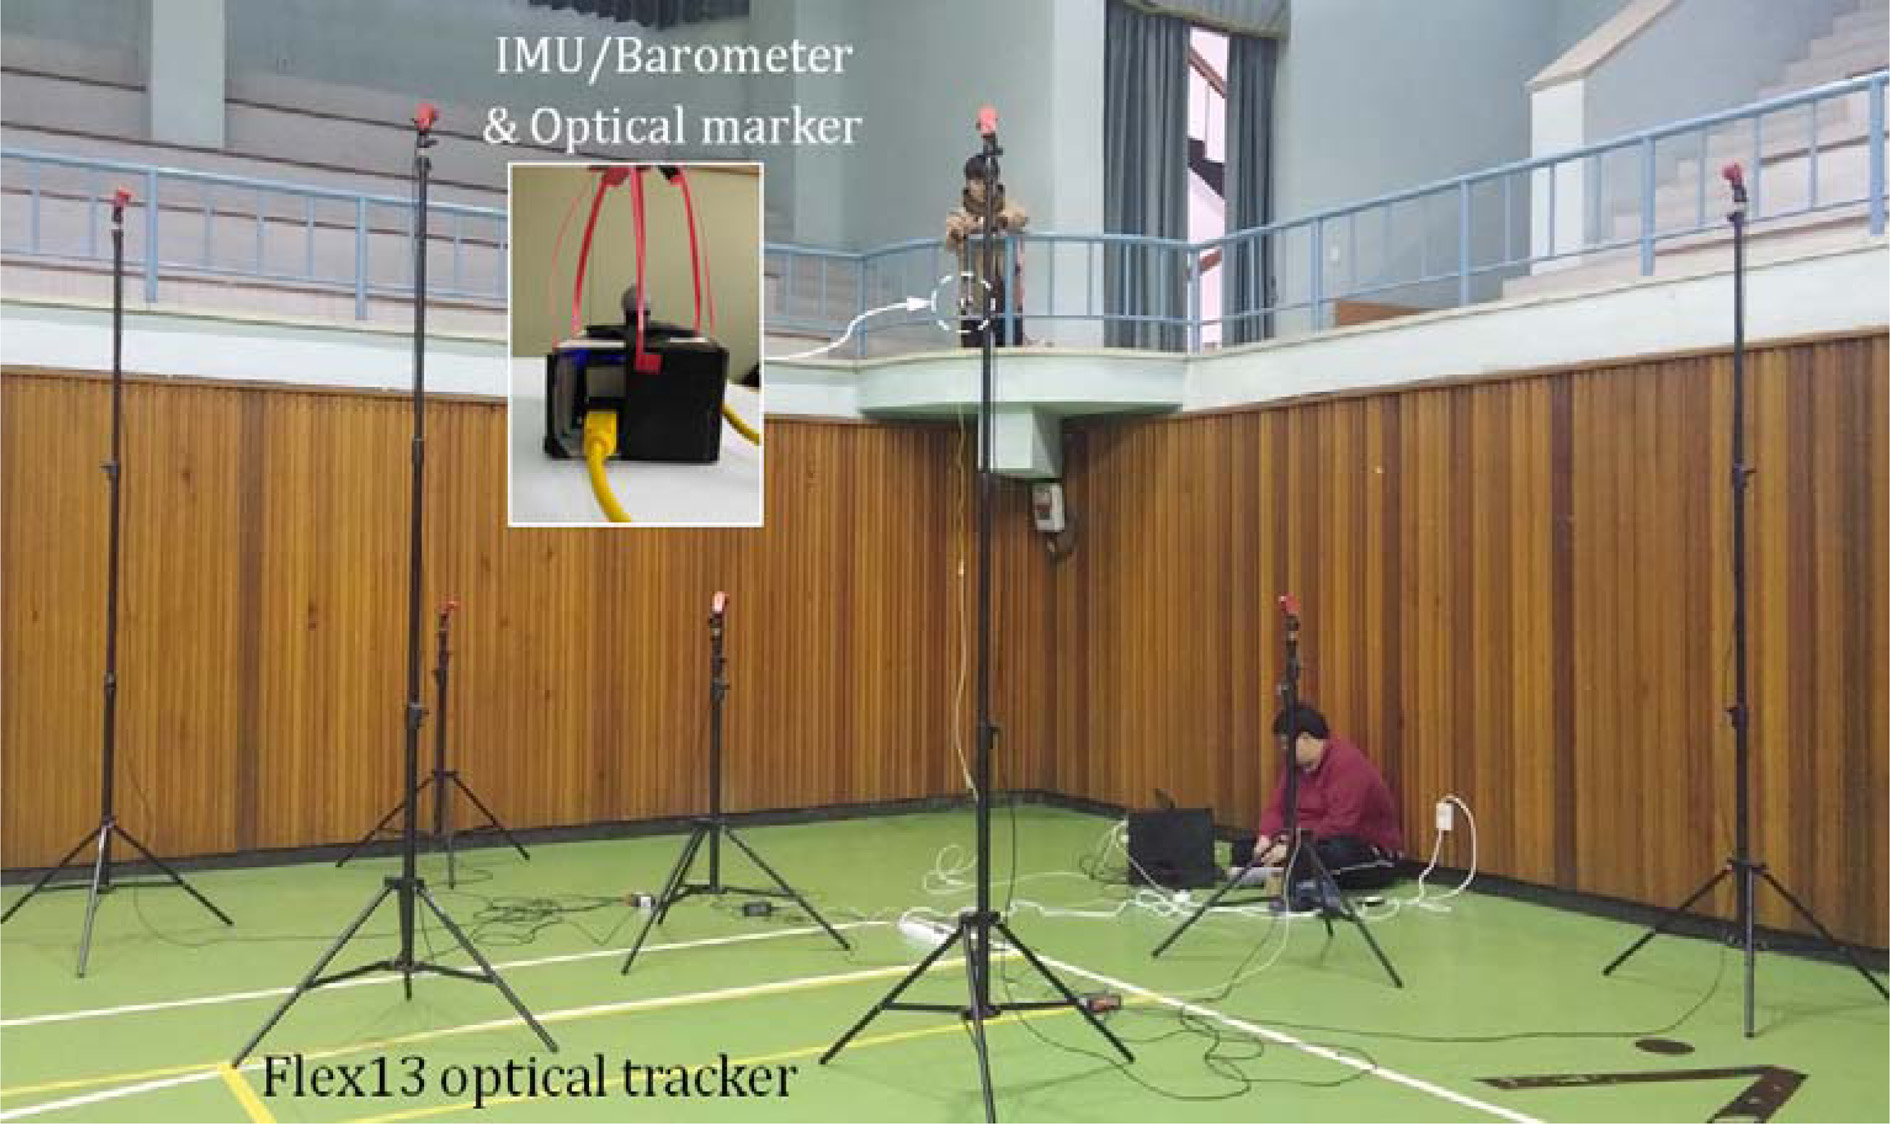
\includegraphics[width=2.5in]{fig3}
\caption{Test setup with the Fex 13 optical motion capture system in an indoor gym.}
\label{fig3}
\end{figure}


\begin{figure}[!t]
\centering
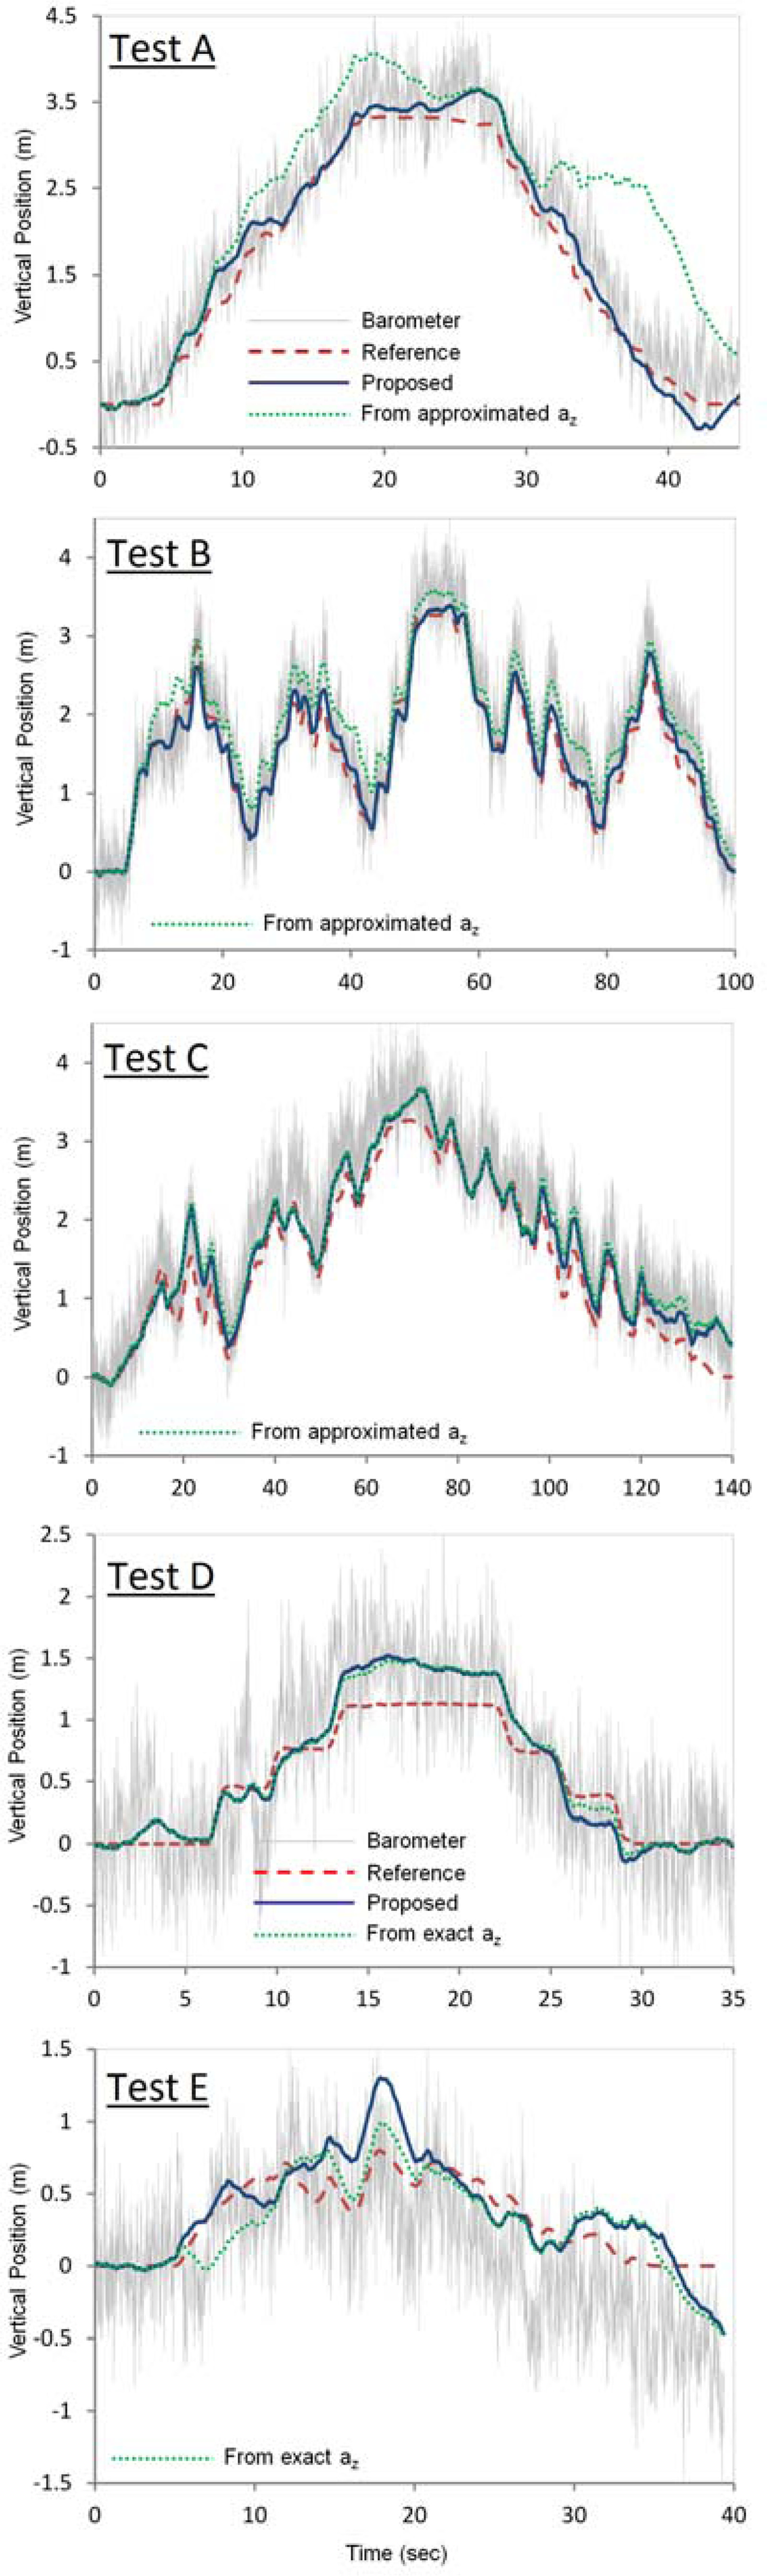
\includegraphics[width=2.5in]{fig4}
\caption{Comparison of vertical position estimations.}
\label{fig4}
\end{figure}


\section{Results}

Table 2 shows the RMSE for each case, and Fig. 4 shows the result of applying CF in the second step.

(Test A - C results) In case of applying $a_{z,app}$ In the case of vertical
motion in which the change of attitude was not large as in Test B or Test C,
since $a_{z,app}$ maintains some accuracy, the vertical displacement estimate
was also obtained more accurately than with the barometer by itself ($s_B$).
However, as in Test A, when the sensor posture changed significantly and the
vertical motion was performed, the estimation accuracy was estimated to be even
larger than the RMSE of $s_B$. The maximum error was 26.2 cm in Test C, and
even less than 30 cm of accuracy was achieved in a displacement test of 3 m or
more. In Test C, it seems that the influence of the large error of the
barometer signal is reflected in the estimated value.

(Test D - E) Overall accuracy was highest for $a_{z,OPT}$, which estimated
vertical displacement based on very accurate vertical acceleration. However,
the proposed $a_{z,KF}$ method also showed very high accuracy ($a_{z,OPT}$ is
comparable to the analytical comparison, which can not be obtained with the
IMU-barometer system), averaging 1.4 cm averaged over $a_{z,OPT}$ method.
The $a_{z,app}$ method showed very different results depending on the degree of
sensor posture maintained.  For example, as in Test D, the RMSE was less than 20
cm in accuracy for a motion that included a stationary state with no change in
posture.

The barometer signal functions to prevent drift errors and ultimately
determines the direction of the estimated value. In other words, It is
inevitable that the estimated value is also affected if the error increases to
the abnormal barometer signal which depends on the barometer signal to prevent
drift error.  For example, if you look at the portion after 35 seconds in Test
E, the sensor stopped at the 0 m initial position, but the barometer signal
continued to drop, and you can see how the estimated value tracks it. Therefore, in
order to improve the estimation performance, it is necessary to improve the
performance of the barometer itself.

In conclusion, there was no performance difference between CF and KF in all
five tests.  However, considering the amount of calculation (CF / KF
calculation ratio = 12.5\%), it can be concluded that CF is advantageous
overall. The proposed method has an average RMSE of 19.7 cm, which is 55\%
better than the RMSE 43.4 cm of the barometer signal itself.  In [2], vertical
acceleration estimation with Kalman filter and vertical displacement estimation
with Kalman filter (ie, two-stage Kalman / Kalman filter) and average RMSE 27.4
cm was obtained.

\section{Review and Conclusion}

In this paper, a two-stage Kalman / complementary filter for vertical
displacement estimation based on IMU-barometer was proposed. The Kalman filter
(KF) for estimating the vertical acceleration in the first stage estimates the
vertical acceleration via the tilt posture using the 6-axis IMU signal. In the
second-stage complementary filter (CF), vertical displacement and vertical
velocity are estimated using vertical acceleration and barometric signal
transmitted through the first Kalman filter. The following conclusions are
drawn from various experiments.

1. In the vertical displacement estimation filter using the vertical
acceleration estimate and the barometric signal, there was almost no difference
in accuracy between KF and CF (absolute difference value average 0.15 cm).
However, considering the calculation time, the CF method is much faster than KF
(8 times), so we conclude that the CF adopted by this paper is better.

2. Unless there is little change in attitude, approximated vertical
acceleration estimation using only an accelerometer is inadequate for use in
estimating vertical displacement (despite the ease of sensor configuration and
method).

3. In the vertical acceleration estimation based on the IMU-barometric fusion
sensor, the performance of the barometer has a great influence on the
estimation accuracy, and it seems that there is a limit to improving the accuracy
through the IMU.  However, in comparison with the barometer signal error of
43.4cm average RMSE, the average RMSE error of the proposed method was 19.7cm.

In this paper, we proposed a method to efficiently improve the accuracy of
vertical displacement estimation through IMU-barometric fusion. It can be
widely applied to sports science and ship VDR (voyage data recorder) as well as
pedestrian navigation and fall detection.

\section*{Acknowledgments}

The work described in this paper was carried out with support from the Small
and Medium Business Administration's research village project (C0301478) and
the Korea Research Foundation (NRF-2015R1C1A1A02036373) of the Institute for
Future Creation Sciences.

\begin{table}[tp]
\caption{Specification of GYU-87 IMU-Barometer system.}
\vspace*{-5mm}
\label{table:levels}
\centering
\begin{tabular}{llll}
\\ \toprule
& Accelerometer & Gyroscope & Barometer\\ \midrule

Model 
& \multicolumn{1}{ p{1.5cm} }{\centering Invensense \\ MPU-6050} 
& \multicolumn{1}{ p{1.5cm} }{\centering Invensense \\ MPU-6050} 
& \multicolumn{1}{ p{1.5cm} }{\centering Bosch \\ BMP 180} \\
\hline\\

Full-Scale Range 
& $\pm 2 \sim 16 g$ 
& \multicolumn{1}{ p{1.5cm} }{\centering $\pm 250 \sim$ \\ 2000 deg/s} 
& \multicolumn{1}{ p{1.5cm} }{\centering $\pm 300 \sim$ \\ 1100 hPa} \\
\hline\\

Sensitivity
& \multicolumn{1}{ p{1.5cm} }{\centering $0.000061 \sim$ \\ 0.0049 g} 
& \multicolumn{1}{ p{1.5cm} }{\centering $0.0076 \sim$ \\ 0.061 deg/s} 
& \multicolumn{1}{ p{1.5cm} }{\centering 0.0015 hPa} \\
\hline\\

\multicolumn{1}{ p{2cm} }{\centering Max. Sampling\\ Rate} 
& 1000 Hz
& 8000 Hz
& 128 Hz \\
\hline\\

Digital Resolution
& 16 bit
& 16 bit
& 19 bit\\
\hline

\end{tabular}
\end{table}  

\renewcommand{\arraystretch}{1.5}

\begin{table}[tp]
    \caption{RMSE (root mean squared error) of raw barometer signal and estimations of each case
    (unit: cm)}
\vspace*{-5mm}
\label{table:rmse}
\centering
\begin{tabular}{llllll}
\\ \toprule
\textbf{Test} & $S_B$ & \textbf{Filter} & $a_{z,OPT}$ & $a_{z,KF}$ & $a_{z,app}$ \\ \midrule
Test A & 41.7 & CF & N/A & 19.9 & 86.8\\ \hline &  & KF & N/A & 19.8 & 86.9\\ \hline
Test B & 42.0 & CF & N/A & 13.9 & 37.4\\ \hline &  & KF & N/A & 13.8 & 37.4\\ \hline
Test C & 50.4 & CF & N/A & 26.2 & 32.4\\ \hline &  & KF & N/A & 26.2 & 32.4\\ \hline
Test D & 40.8 & CF & 16.8 & 18.5 & 18.2 \\ \hline &  & KF & 16.3 & 18.1 & 18.6\\ \hline
Test E & 42.2 & CF & 18.7 & 19.9 & 32.1 \\ \hline &  & KF & 18.7 & 19.8 & 32.0\\ \hline
Average & 43.4 & & 17.8 & 19.7 & 41.4 \\ \hline &  & & 17.5 & 19.5 & 41.5\\ \hline
\\
\\
\end{tabular}
\end{table}  

\begin{thebibliography}{1}

    \bibitem{Gasior}
        P. G\k{a}sior, S. Gardecki, J. Go\'{s}li\'{n}ski, and W. Giernacki,
        ``Estimation of altitude and vertical velocity for multirotor
        aerial vehicle using Kalman filter,'' in \emph{Recent Advances in
        Automation, Robotics and Measuring Techniques}, Vol. 267,
        R. Szewczyk, C. Zieli\'{n}ski, and M. Kaliczy\'{n}ska, Eds. Hei-
        delberg, Germany: Springer International Publishing, 2014,
        pp. 377-385.

    \bibitem{Zihajehzadeh}
        S. Zihajehzadeh, T. J. Lee, J. K. Lee, R. Hoskinson, and E.
        J. Park, ``Integration of MEMS inertial and pressure sensors
        for vertical trajectory determination,'' \emph{IEEE Trans. Instrum.
        Meas.}, Vol. 64, No. 3, pp. 804-814, 2015.

    \bibitem{Svbavensky}
        O. \v{S}v\'{a}bensk\'{y}, J. Weigel, and R. Machotka, ''On GPS
        heighting in local networks,'' \emph{Acta Geodyn. Geomater.}, Vol.
        3, No. 143, pp. 39-43,Jun. 2006.

    \bibitem{Son}
        Y. B. Son, and S. Y. Oh, ``A barometer-IMU fusion method
        for vertical velocity and height estimation,'' \emph{IEEE Proc. of
        Sensors}, pp. 1-4, Busan, Korea, 2015.

    \bibitem{Sabatini}
        A. M. Sabatini and V. Genovese, ``A sensor fusion method
        for tracking vertical velocity and height based on inertial
        and barometric altimeter measurements,'' \emph{Sensors}, Vol. 14,
        No. 8, pp. 13324-13347, 2014.

    \bibitem{Pierleoni}
        P. Pierleoni, A. Belli, L. Palma, L. Pernini, and S. Valenti,
        ``An accurate device for real-time altitude estimaion using
        data fusion algorithms,'' \emph{Proc. of 2014 IEEE/ASME 10th
        Int'l Conf. on MESA.}, pp.1-5, Senigallia, Italy, 2014.

    \bibitem{Tanigawa}
        M. Tanigawa, H. Luinge, L. Schipper, P. Slycke, ``Drift-free
        dynamic height sensor using MEMS IMU aided by MEMS
        pressure sensor,'' \emph{Proc. 5th Workshop on Positioning, Nav-
        igation and Communication}, pp. 191-196, Hannover, Ger-
        many, 2008.

    \bibitem{Kim}
        Y. Kim, Y. Hwang, S. Choi and J. Lee, ``Height estimation
        scheme of low-cost pedestrian dead-reckoning system using
        Kalman filter and walk condition estimation algorithm,''
        \emph{Proc. of IEEE/ASME International Conf. on AIM.}, pp.1492-
        1497, Wollongong, Australia, 2013.

    \bibitem{Bianchi}
        F. Bianchi, S. J. Redmond, M. R. Narayanan, S. Cerutti, and
        N. H. Lovell, ``Barometric pressure and triaxial acceler-
        ometry-based falls event detection,'' \emph{IEEE Trans. Neural
        Sys. Rehab. Eng.}, Vol. 18, No. 6, pp. 619-627, 2010.

    \bibitem{Lee}
         J. K. Lee, E. J. Park, and S. N. Robinovitch, ``Estimation of
        attitude and external acceleration using inertial sensor mea-
        surement during various dynamic conditions'' \emph{IEEE Trans.
        Instrum. Meas.}, Vol. 61, No. 8, pp. 2262-2273, 2012.

    \bibitem{Walter}
         T. Walter, and J. R, Higgins, ``A comparison of comple-
        mentary and Kalman filtering,'' \emph{IEEE Trans. Aerosp. Elec-
        tron. Syst.}, Vol. AES-11, No. 3, pp. 321-325, 1975.

    \bibitem{Sabatini}
         A. M. Sabatini and V. Genovese, ``A stochastic approach to
        noise modeling for barometric altimeters,'' \emph{Sensors}, Vol. 13,
        No. 11, pp. 15692-15707, 2013.

    \bibitem{Degen}
         T. Degen, H. Jaeckel, M. Rufer, and S. Wyss, ``SPEEDY: a
        fall detector in a wrist watch'' in \emph{Proc. 7th IEEE Int. Sym-
        posium on Wearable Computing}, pp. 184-187, 2003.

    \end{thebibliography}


\end{document}
